\documentclass[11pt,a4paper]{article}

% --- Mathematics (must precede unicode-math) ---
\usepackage{amsmath}
\usepackage{mathtools}

% --- Fonts (lualatex) ---
\usepackage{fontspec}
\usepackage{unicode-math}
\setmathfont{KpMath-Regular.otf}
\setmathfont{KpMath-Bold.otf}[version=bold]

\usepackage{microtype}
\usepackage[dvipsnames]{xcolor}
\usepackage[margin=25mm, top=30mm, bottom=30mm]{geometry}

\usepackage{fancyhdr}
\pagestyle{fancy}
\fancyhf{}
\fancyhead[L]{\small\itshape Polynomial Voxels on an Octree: archived material}
\fancyhead[R]{\small\itshape Nestor (2026), archive}
\fancyfoot[C]{\thepage}
\renewcommand{\headrulewidth}{0.4pt}
\renewcommand{\footrulewidth}{0pt}

\setcounter{secnumdepth}{3}
\usepackage{booktabs}
\usepackage{array}
\usepackage{graphicx}
\usepackage{placeins}
\usepackage[numbers,sort&compress]{natbib}
\usepackage[font=small, labelfont=bf, labelsep=period]{caption}
\usepackage{setspace}
\setstretch{1.15}
\setlength{\parskip}{0.4em}
\usepackage[colorlinks=true, linkcolor=blue!60!black,
            citecolor=blue!60!black, urlcolor=blue!60!black]{hyperref}

% --- Macros ---
\newcommand{\bk}{\mathbf{k}}
\newcommand{\bx}{\mathbf{x}}
\newcommand{\bK}{\mathbf{K}}
\newcommand{\bD}{\boldsymbol{\Delta}}
\newcommand{\cE}{\mathcal{E}}
% the differential of every integral and derivative is upright; an italic d is the side of a cell
\newcommand{\dd}{\mathrm{d}}

\title{\bfseries Polynomial Voxels on an Octree\\[4pt]
\large Blocks between Unequal Cells, Refinement by the Two-Term Error Estimate,\\
and the Basis for a Medium that is Piecewise Constant on the Leaves}
\author{T. M. Nestor\\[2pt]\small Independent researcher, Australia}
\date{Archive, 9 October 2026}

\begin{document}
\maketitle

\begin{abstract}
\noindent
This document archives the octree material removed from the paper on the error of polynomial voxels
\citep{NestorError2026} when that paper was narrowed to the error analysis on uniform grids. It is kept
as a record, not as a paper. It holds the octree itself (leaves of different sizes, the exact blocks
between them as sums of blocks between equal cells, and their reduction by the symmetry of the cube), the
two-term error law measured on trees, the refinement rule built on the two terms and its test on a sphere
with a localised feature, the test on a medium that is piecewise constant on the leaves, and a summary of
the two-scale Galerkin refinement studied afterwards. Why the line was set aside is stated first
(\S\ref{sec:why}). The error law that the refinement uses is that of \citet{NestorError2026}, whose
equations and sections are cited here in words.
\end{abstract}

\section{Why the octree was set aside}\label{sec:why}

\begin{itemize}
\item \emph{Size.} The tree solver is dense and stops near $20\,000$ unknowns: about $2200$ constant
leaves or $550$ degree-one leaves. Every result below is on a small body. A tree of $344$ leaves of four
sizes is assembled and solved in about three minutes; an equal-cell block costs about $50$\,ms.
\item \emph{A fast solver is a project of its own.} Its parts are published: the fast multipole method
for volume potentials on an octree \citep{Malhotra2016}, the elastic kernels in fast multipole methods for
boundary integral equations \citep{Fujiwara2000,Chaillat2008}, and, for cells mapped to a uniform grid, the
adaptive integral method \citep{Bleszynski1996}. None is implemented here.
\item \emph{The refinement did not improve further.} The two-scale Galerkin indicator of
\S\ref{sec:twoscale} builds the trees of the two-term rule and reaches the same accuracy, at the cost of a
solve per step where the two-term rule needs none.
\item \emph{The largest gain is self-consistent.} The factor of $65$ of \S\ref{sec:blocky} is against a
reference computed by the same scheme with degree-two fields, on a body whose field is not smooth near
the edges and corners of its cubes.
\item \emph{Uniform grids do well.} Uniform grids of Legendre cells, applied by fast Fourier transforms,
reach high accuracy on a graded sphere without a tree \citep{NestorCoupling2026}; the tree paid only where
the variation of the medium filled a few per cent of the volume.
\end{itemize}

\section{The octree}\label{sec:setting}

\paragraph{Leaves.} The body is covered by cubes, the leaves of an octree: leaf $\ell$ has centre
$\bx_\ell$ and half-width $h_\ell$ (side $d_\ell=2h_\ell$), and the half-widths are in ratios that are
powers of two. With $\boldsymbol\xi=(\bx-\bx_\ell)/h_\ell$ the local coordinate, the leaf carries the
nine-component state (displacement and strain) in the Legendre products
$Q_a(\boldsymbol\xi)=P_{a_1}(\xi_1)P_{a_2}(\xi_2)P_{a_3}(\xi_3)$ of total degree $|a|=a_1+a_2+a_3\le p_\ell$,
which is $1$, $4$ or $10$ functions for $p_\ell=0$, $1$ or $2$, and the contrast in the same products to
degree $r_\ell$. The two degrees may differ from leaf to leaf. A leaf with $p=r=0$ is a Haar cell: a
constant medium and a constant field. We call it a constant cell, a leaf with $p=r=1$ a degree-one cell
(the constant and the three linear polynomials, $\xi_1$, $\xi_2$, $\xi_3$), and a leaf with $p=r=2$ a
degree-two cell (those four and the six quadratic products, $P_2(\xi_i)$ and $\xi_i\xi_j$ with $i<j$; ten in all).

\paragraph{The system.} Tested with the same functions, the volume integral equation becomes
\begin{equation}\label{eq:system}
  M_\ell\,\psi_\ell-\sum_{m}\bK(\ell,m)\,E_m\,\psi_m=\langle Q,\psi^0\rangle_\ell ,
\end{equation}
with $\psi_\ell$ the coefficients of the state in leaf $\ell$, $M_\ell$ the Gram matrix of its
functions, $E_m$ the projected contrast of leaf $m$ acting on its field, $\psi^0$ the incident wave and
$\bK(\ell,m)$ the block that couples the two leaves: the Green's tensor integrated against the functions
of both \citep{NestorContinuum2026}.

\paragraph{Blocks between leaves of different sizes.} A polynomial on a cube is a polynomial of the
same degree on each of the cube's descendants, so the block between a large leaf and a small one is an
exact, finite sum of blocks between equal cells: the large leaf is replaced by its descendants at the
size of the small one, with its polynomials re-expanded (Figure~\ref{fig:octree}c). No integral is needed beyond those between equal cells. This is the two-scale
relation of the multiwavelet basis \citep{Alpert1993}. Against six-dimensional quadrature these blocks agree to $10^{-9}$ for leaves one and two
levels apart, and on a tree whose leaves are all equal the solver reproduces the uniform solver to
$10^{-11}$.

\paragraph{Symmetry.} Two pairs of leaves whose relative positions are images of one another under a
reflection or a permutation of the axes have blocks related by the representation of that operation on
the polynomials and on the nine components, whatever the two sizes, because the operation acts on both
cubes alike. One block is therefore computed for each orbit of the cube's group of $48$ operations.
On a tree of $344$ leaves of three sizes this reduced the assembly from $125$\,s to $65$\,s with an
unchanged solution, and made trees with four sizes practicable.

\begin{figure}[htbp]
\centering
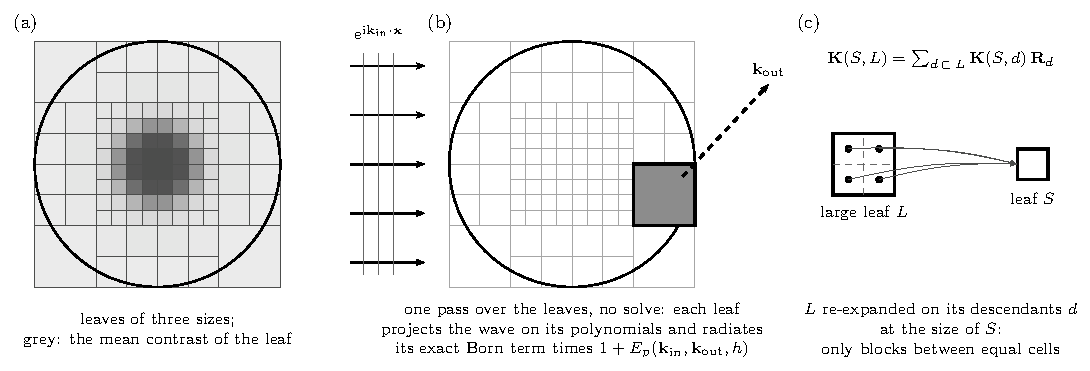
\includegraphics[width=\linewidth]{figures/fig_octree.pdf}
\caption{The octree, drawn as its two-dimensional slice. (a)~The leaves on a body with a weak halo and
a compact graded feature, refined where the feature's contrast varies, in three sizes; the grey level
is the leaf's mean contrast, which the leaf holds as a polynomial of degree $r$. (b)~The term of first
order needs no solve: each leaf holds the projection of the incident wave onto its own polynomials and
radiates its exact Born field times the wave factor $1+E_p$ of \citet{NestorError2026}, which depends only on
the leaf's half-width and the two wavevectors, so the whole
term is one pass over the leaves. (c)~The block between a large leaf $L$ and a small leaf $S$ is the
sum of the blocks between $S$ and the descendants $d$ of $L$ at the size of $S$, with the polynomials
of $L$ re-expanded on them ($\mathbf{R}_d$): only blocks between equal cells are ever integrated. The
tree is generated by \texttt{figures/make\_fig\_octree.py}.}\label{fig:octree}
\end{figure}

\section{The two-term law on trees}\label{sec:treelaw}

The law of \citet{NestorError2026}, that the error of the far field less its first-order error is the
nonlinear fraction of the response times the relative projection error $\cE_r$ of the medium, times a
factor of order one, was measured on uniform grids and on trees alike. The full table is kept here; the
error paper keeps its uniform rows. The test body is a sphere of radius $a$ with a uniform core of radius
$0.75a$ and a shell across which the contrast falls smoothly to zero, at $k_Sa=0.5$; the error is the
largest difference of the far field from the exact one over nine scattering angles, relative to its peak.
\begin{table}[htbp]
\centering
\caption{The error of the far field in two terms, on the sphere with a graded shell. The rest is the
error less the first-order error, which is computed without a solve. $\cE$ is the relative projection
error of the medium at the degree of the cells \citep{NestorError2026}. The nonlinear fraction of the exact response
is $0.0151$.}\label{tab:twoterm}
\small
\begin{tabular}{@{}llrccc@{}}
\toprule
cells & grid & leaves & error & error / $\cE$ & rest / $\cE$ \\
\midrule
constant ($p=r=0$) & uniform & $64$   & $8.17\times10^{-3}$ & $0.0309$ & $0.0149$ \\
 & uniform & $184$  & $3.18\times10^{-3}$ & $0.0235$ & $0.0151$ \\
 & uniform & $408$  & $1.61\times10^{-3}$ & $0.0196$ & $0.0154$ \\
 & uniform & $1256$ & $6.77\times10^{-4}$ & $0.0166$ & $0.0158$ \\
 & tree    & $232$  & $3.29\times10^{-3}$ & $0.0321$ & $0.0152$ \\
 & tree    & $856$  & $9.28\times10^{-4}$ & $0.0210$ & $0.0152$ \\
 & tree    & $1360$ & $6.03\times10^{-4}$ & $0.0210$ & $0.0151$ \\
 & tree    & $1696$ & $5.75\times10^{-4}$ & $0.0222$ & $0.0151$ \\
\midrule
degree one ($p=r=1$) & uniform & $64$  & $8.99\times10^{-4}$ & $0.0147$ & $0.0148$ \\
 & uniform & $184$ & $4.62\times10^{-4}$ & $0.0146$ & $0.0146$ \\
 & uniform & $408$ & $2.20\times10^{-4}$ & $0.0146$ & $0.0146$ \\
 & tree    & $184$ & $5.16\times10^{-4}$ & $0.0142$ & $0.0148$ \\
 & tree    & $352$ & $2.20\times10^{-4}$ & $0.0146$ & $0.0145$ \\
\bottomrule
\end{tabular}
\end{table}
For constant cells the ratio of error to projection error varies by a factor of $1.93$ across the
grids; the rest over the projection error varies by $1.06$, and it is $0.0151$ to $0.0152$ on all four
trees. For degree-one cells the first-order error is small and both ratios are near $0.0146$. The constant
is close to the nonlinear fraction of the exact response, $\nu=\lvert u-T_1\rvert/\lvert u\rvert=0.0151$, on trees as on uniform grids.
\section{Refinement by the two terms}\label{sec:refine}

\paragraph{The rule.} Each leaf has two indicators, both computed before any solve. The \emph{medium}
indicator is the nonlinear fraction $\nu$ times the leaf's share of the projection error,
$\nu\int_\ell(f-\Pi_rf)^2\,\dd V/\int f^2\,\dd V$. The \emph{wave} indicator is the leaf's own
first-order error, computed without a solve \citep{NestorError2026}, relative to the peak of the Born far field. A leaf is split into
its eight children while the sum of the two exceeds a tolerance. The nonlinear fraction is estimated on a
coarse tree that resolves the medium, from two products with its matrix and no
solve \citep{NestorError2026}. The experiments below were first run with the earlier estimate, from one solve on
that tree; the trees and their errors are the same with either, since $\nu$ enters the rule only through
the medium indicator and the two estimates differ by up to a fifth, and only the predicted errors
change. The predicted error of a tree is the first-order error of the whole tree, summed over the leaves
as complex amplitudes, plus $\nu\,\cE_r$. It uses no reference solution.

\paragraph{A localised feature.} The test body is a sphere of radius $a$ whose contrast is a weak
halo, falling smoothly from $5\%$ of the central value to zero across the whole radius, plus a
compact feature in which it falls from the central value to the halo between $0.1a$ and $0.3a$: under
$3\%$ of the volume. Its exact solution is known. At $k_Sa=1$, with leaves no smaller than $a/32$, the
errors are those of Table~\ref{tab:refine}. The rule that uses the medium alone refines a leaf while
its share of the projection error exceeds a tolerance.
\begin{table}[htbp]
\centering
\caption{The localised feature: leaves, the error predicted without a reference, and the error against
the exact solution. The nonlinear fraction estimated on a coarse tree, with no solve, is
$0.0059$ for constant and for degree-one cells, the exact value; the earlier estimate from a solve was
$0.0051$ for constant cells.}\label{tab:refine}
\small
\begin{tabular}{@{}llrcc@{}}
\toprule
cells & grid & leaves & predicted & error \\
\midrule
constant & uniform & $408$ & $1.15\times10^{-2}$ & $7.15\times10^{-3}$ \\
 & uniform & $1256$ & $4.50\times10^{-3}$ & $2.92\times10^{-3}$ \\
 & medium alone & $344$ & $1.61\times10^{-2}$ & $1.55\times10^{-2}$ \\
 & medium alone & $512$ & $1.57\times10^{-2}$ & $1.53\times10^{-2}$ \\
 & medium alone & $736$ & $5.96\times10^{-3}$ & $5.49\times10^{-3}$ \\
 & two terms & $260$ & $8.31\times10^{-3}$ & $7.18\times10^{-3}$ \\
 & two terms & $372$ & $6.93\times10^{-3}$ & $5.38\times10^{-3}$ \\
 & two terms & $752$ & $4.53\times10^{-3}$ & $3.78\times10^{-3}$ \\
 & two terms & $1780$ & $2.22\times10^{-3}$ & $1.75\times10^{-3}$ \\
\midrule
degree one & uniform & $184$ & $2.86\times10^{-3}$ & $2.73\times10^{-3}$ \\
 & uniform & $408$ & $8.36\times10^{-4}$ & $6.77\times10^{-4}$ \\
 & medium alone & $176$ & $2.44\times10^{-4}$ & $2.47\times10^{-4}$ \\
 & medium alone & $344$ & $1.95\times10^{-4}$ & $1.96\times10^{-4}$ \\
 & two terms & $260$ & $1.73\times10^{-4}$ & $1.68\times10^{-4}$ \\
 & two terms & $336$ & $1.57\times10^{-4}$ & $1.66\times10^{-4}$ \\
 & two terms & $452$ & $1.09\times10^{-4}$ & $1.14\times10^{-4}$ \\
\bottomrule
\end{tabular}
\end{table}

\paragraph{Constant cells.} The rule that uses the medium alone fails: with $512$ leaves its error is
twice that of the uniform grid of $408$ cells. It refines the feature and leaves the halo coarse, and
the halo is where the first-order error is, in leaves whose medium is too smooth for the rule to see.
The rule with two terms sees it. Its tree of $260$ leaves has the error of the uniform grid of $408$,
and against the trend of the uniform grids its trees have the same error with about $35\%$ fewer cells
at the coarse end and an error $15$ to $20\%$ lower at the fine end. The saving is modest, and the
reason is the cell: a constant field has a second-order error in every leaf, so the halo needs cells
however smooth its medium is.

\paragraph{Degree-one cells.} Here the tree pays. The tree of $176$ leaves has eleven times less error than
the uniform grid of $184$ cells. By the trend of the two uniform grids its error would need about $730$
uniform cells, four times as many, and that of the tree of $452$ leaves about $1130$; these uniform
equivalents are extrapolated, not computed. The fourth-order error of a degree-one field lets the halo stay
coarse, and the tree then follows the medium. The two-term rule improves on the medium alone by about
$15\%$ at about $340$ leaves.

\paragraph{The prediction.} The predicted error is above the true error on all eleven grids of constant
cells computed for this body (nine of them in Table~\ref{tab:refine}), by $3\%$ to $61\%$. For degree-one
cells the ratio of predicted to true is $0.95$ to $1.23$ on nine grids: close, but not a bound.

\section{A medium that is piecewise constant on the leaves}\label{sec:blocky}

The pairing of a constant medium with a
polynomial field belongs to the medium that is constant in each leaf. The test body is a cube of
half-side $B$ with a uniform contrast a quarter of the central value, holding at its centre a cube of
half-side $B/4$ with the full contrast, at $k_SB=2$. A tree of $120$ leaves represents it exactly with
one constant per leaf ($\cE_0=0$): $56$ leaves of half-width $B/4$ and $64$ of half-width $B/8$. The
uniform grid that does the same has $512$ cells. No exact solution is known for this body; the
reference is the tree with degree-two fields, whose own first-order error is predicted to be
$2\times10^{-7}$ (Table~\ref{tab:blocky}).
\begin{table}[htbp]
\centering
\caption{A cube within a cube, the contrast constant in every leaf. The first-order error is predicted
without a solve; the error is against the tree with degree-two fields. In the last two rows the faces of
the inner cube fall inside the cells of the grid.}\label{tab:blocky}
\small
\begin{tabular}{@{}lrrcc@{}}
\toprule
grid and field & cells & unknowns & predicted & error \\
\midrule
tree, constant field & $120$ & $1080$ & $1.54\times10^{-2}$ & $1.53\times10^{-2}$ \\
tree, degree one in the $56$ large leaves & $120$ & $2592$ & $3.24\times10^{-3}$ & $3.21\times10^{-3}$ \\
tree, degree-one field & $120$ & $4320$ & $8.07\times10^{-5}$ & $8.42\times10^{-5}$ \\
uniform, constant field & $512$ & $4608$ & $5.54\times10^{-3}$ & $5.51\times10^{-3}$ \\
uniform, degree-one field & $512$ & $18432$ & $8.17\times10^{-6}$ & $9.25\times10^{-6}$ \\
\midrule
uniform, constant field & $64$ & $576$ & $1.81\times10^{-2}$ & $1.79\times10^{-2}$ \\
uniform, degree-one field & $64$ & $2304$ & $3.01\times10^{-2}$ & $2.92\times10^{-2}$ \\
\bottomrule
\end{tabular}
\end{table}
With the medium exact there is no second term, and the first-order prediction is within $13\%$ of the
measured error in all seven cases and within $4\%$ in five. The tree with a degree-one field has an error
of $8.4\times10^{-5}$ with $4320$ unknowns; the uniform grid of constant cells has $5.5\times10^{-3}$
with $4608$: $65$ times more. Raising the field to degree one in the large leaves alone lowers the tree's
error from $1.5\times10^{-2}$ to $3.2\times10^{-3}$: a large leaf needs a richer basis for the
wavefield, not for the medium. And where the faces of the inner cube fall inside cells, the degree-one
field is worse than the constant one, as on the smooth body; for the scalar problem
\citet{Anderson2026} likewise find that high order is lost at jumps of the medium unless the grid
follows them.

\paragraph{The choice.} The two cases give the rule. Where the medium is piecewise constant and the
tree can follow its interfaces, hold it constant in each leaf and spend the degree on the field.
Where it varies smoothly, give the medium and the field the same degree and let the tree follow the
medium. In both the error is predicted before the solve.

\section{The two-scale Galerkin refinement}\label{sec:twoscale}

After the two-term rule, a refinement indicator was derived from the two nested Galerkin problems of a
tree and of its children (\path{docs/2026-10-09-two-scale-galerkin.md}). The residual of the prolonged
coarse solution splits exactly into a part driven by the detail of the medium and a part driven by the
multiwavelet detail of the field, and the error of the far field is a sum of their shares, cell by cell,
weighted by the adjoint solution. On a graded sphere the identities hold to $10^{-13}$, the two-scale
difference measures the coarse error to $7\%$, as fourth-order convergence predicts, and a two-level
estimate, with one coarse solve and one fine product, gives the error to $0.03$ to $0.14\%$
(\path{scripts/derive_two_scale_galerkin.py}).

On an octree (degree-one cells, $k_Sa=1$, leaves no smaller than $a/32$, the fine operator applied by fast
Fourier transform on the finest uniform grid; \path{scripts/pilot_octree_two_scale_refinement.py}), the
indicator with a tolerance per leaf builds the trees of the two-term rule, and marking by the D\"orfler
criterion reaches the same band (Table~\ref{tab:twoscale}).
\begin{table}[htbp]
\centering
\caption{Refinement on the localised feature of \S\ref{sec:refine}, degree-one cells: leaves and error
against the exact solution.}\label{tab:twoscale}
\small
\setlength{\tabcolsep}{3pt}
\begin{tabular}{@{}lccccc@{}}
\toprule
leaves & \multicolumn{2}{c}{two-scale indicator} & two-term & medium alone & uniform \\
 & tolerance per leaf & D\"orfler, $\theta=0.5$ & & & \\
\midrule
$120$--$184$ & $120$: $6.8\times10^{-4}$ & $134$: $5.4\times10^{-4}$ & & $176$: $2.47\times10^{-4}$ & $184$: $2.73\times10^{-3}$ \\
$218$--$260$ & $260$: $1.68\times10^{-4}$ & $218$: $2.9\times10^{-4}$ & $260$: $1.68\times10^{-4}$ & & \\
$336$--$344$ & $344$: $1.66\times10^{-4}$ & $337$: $1.74\times10^{-4}$ & $336$: $1.66\times10^{-4}$ & $344$: $1.96\times10^{-4}$ & \\
$408$--$533$ & & $533$: $1.19\times10^{-4}$ & $452$: $1.14\times10^{-4}$ & & $408$: $6.8\times10^{-4}$ \\
\bottomrule
\end{tabular}
\end{table}
Neither form improves on the two-term rule on this body. The two-scale difference, which needs no
reference, is $73$ to $97\%$ of the true error on trees above $100$ leaves, but each step needs a coarse
solve, a fine product and a second coarse solve, four to five minutes here, where the two-term rule needs
no solve.


\section{Status of this material}\label{sec:status}

\begin{itemize}
\item \emph{Established against exact solutions, by one implementation.} The law on trees
(Table~\ref{tab:twoterm}) and the refinement (Table~\ref{tab:refine}): one frequency each, two bodies,
both spheres with radial profiles.
\item \emph{Self-consistent only.} The cube within a cube (Table~\ref{tab:blocky}) has no exact
solution; its reference is the same scheme with degree-two fields.
\item \emph{Not a bound.} The predicted error exceeded the true error for constant cells in every case,
but fell $5\%$ below it for degree-one cells.
\item \emph{Earlier work.} The adaptive solvers of \citet{Ambikasaran2015} and \citet{Malhotra2016} have
not been read in full for an estimate that relates their refinement tolerance to the error of the
solution.
\end{itemize}

\vfill
\noindent\rule{\linewidth}{0.4pt}\\
{\footnotesize The octree, its blocks and its solver are \path{cubic_scattering/graded_voxel/octree.py},
with tests in \path{cubic_scattering/tests/test_graded_voxel_octree.py}. Table~\ref{tab:twoterm} is
\path{scripts/measure_octree_two_term.py}; Table~\ref{tab:refine} is
\path{scripts/pilot_octree_two_term_refinement.py}; the constant medium with a richer field is
\path{scripts/pilot_octree_hp_refinement.py}; Table~\ref{tab:blocky} is
\path{scripts/pilot_octree_blocky_body.py}; Table~\ref{tab:twoscale} is
\path{scripts/pilot_octree_two_scale_refinement.py}. Their results are stored in
\path{LatexPDFs/AdaptiveOctree/figures} and \path{scratch/two_scale}.}

\bibliographystyle{unsrtnat}
\bibliography{references}

\end{document}
